\section{DNA}
Nucleic acids are one of the building blocks of life, and are composed of a 
backbone made of a type of sugar, with bases that can bond with one another. 
A series of these bases on a backbone is called a sequence. The 
type of sugar as well as the bases depends on the nucleic acid. 
\subsection{RNA} %NEEDS FIGURES
%RNA is massproduced
Ribonucleic acid (RNA) is a large molecule composed of nitrogenous 
bases nested on a ribose-phosphate backbone. The possible nitrogenous bases, or 
bases for short, 
that can be nested on the backbone are guanine (G), adenine (A), uracil (U) and cytosine 
(C). In nature, the predominant form of RNA are as a single-stranded chain 
that can fold in on itself, bundled with other chains to form a structure. 
This flexibility of the backbone that allows for the chain to fold in on itself 
is possible because the RNA's backbone is composed of a sugar called ribose, 
which is unstable compared to its other form, deoxyribose, used in 
deoxyribonucleic acid (DNA), but is more flexible, allowing the RNA chain to 
bend in ways that DNA can not.\\

The bases found in RNA can form hydrogen bonds with each other, though not all 
bases can form bonds with each other. Bases that can bond with each other are 
guanine with cytosine, and adenine with uracil. These bonds are complementary 
of each other, and forms the structure of each RNA. When 
two bases bond with each other, they will stick to each other 
which changes the form of the RNA chain. However sometimes a base will have no 
complementary base to bond with, causing the base to stick out, giving rise to 
certain characteristic forms. This will be elaborated on in section~\ref{structs}.
%Source: http://en.wikipedia.org/wiki/RNA accessed 18/05-2015 12:10

\subsection{Deoxyribonucleic acid}
%DNA is produced for sharing and is maintained
Deoxyribonucleic acid (DNA) is a large molecule composed of nitrogenous bases 
nested on a deoxyribose-phosphate. DNA is mostly found in nature as helixes, 
where two strands has bonded. Similarly to RNA, DNA has four nitrogenous 
bases, and shares three of the four that RNA have, (guanine, adenine and cytosine). 
However instead of uracil, the fourth base is thymine (T). 

%Source: http://en.wikipedia.org/wiki/DNA accessed 18/05-2015 12:28


\subsection{Secondary Structures of Nucleic Acids}\label{structs}
The secondary structure of a nucleic acid describes how the bases of the 
nucleic acid has bonded. The secondary structure of nucleic acids can change if 
the nucleic acid is damaged or has mutated, causing it to gain or lose 
bases. When two bases bond they hold onto each other, causing bases that 
have no complementary base to bond with to stick out. Below are examples of three 
common secondary structures.\\\\
\textbf{Bulge}\\ 
A bulge occurs when one or more bases have no base to bond with, and these 
bases are surrounded by bases that have bonded. This causes the bases to get 
pushed out slightly, resembling a bulging growth. This type of structure occurs 
when one or more bases has been inserted or deleted. If a base has been 
inserted then it will have no base to bond with, and if a base has been deleted 
then the previously-bonded base will have no base to bond with. Figure~\ref{fig:bulge} shows a bulge.

\begin{figure}[H]
\centering
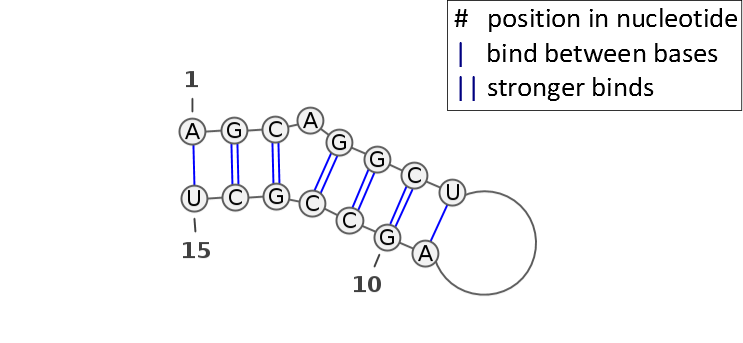
\includegraphics[scale=0.4]{./lib/bulge.png}
\caption{The RNA sequence {\tt AGCAGGCUAGCCGCU}. Note the bulging {\tt A} at position 4.}
\label{fig:bulge}
\end{figure}~
\\
\subsubsection{Interior Loop}
An interior loop is when two or more opposing bases are not complementary and 
can not bond, causing them both to bulge. This occurs when one or more 
consecutive bases mutate to another base. Figure~\ref{fig:int-loop} shows an interior 
loop.
\begin{figure}[h!]
\centering
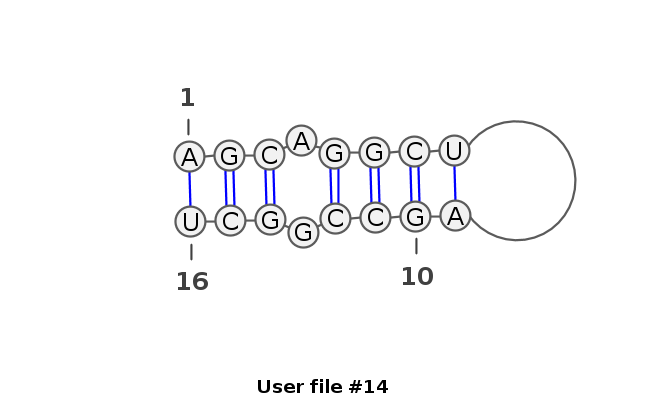
\includegraphics[scale=0.4]{./lib/interior-loop.png}
\caption{The RNA sequence {\tt AGCAGGCUAGCCGGCU}. Note the bulging {\tt A} at position 4 and {\tt G} at position 13
creating a loop inside the bonded strand.}
\label{fig:int-loop}
\end{figure}\\
These interior loops vary in size, and can have differing amount of bases on 
either side of the strands.
\subsubsection{Stem Loop}
A stem loop, also known as a hairpin loop, occurs when a strand bonds with 
itself, but leaves a sequence of bases sticking out that does not bond with anything. 
This kind of loop occurs typically in RNA as they are single-stranded, but may 
happen in single stranded DNA. Figure~\ref{fig:stem-loop} 
shows a stem loop.
\begin{figure}[h!]\centering
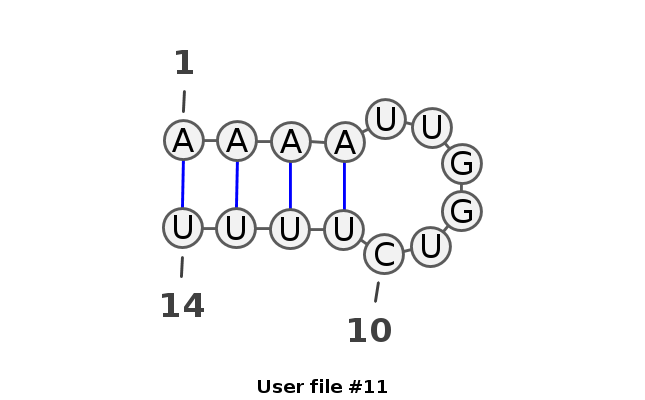
\includegraphics[scale=0.3]{./lib/stem-loop.png}
\caption{A stem loop of the RNA sequence {\tt AAAAUUGGUCUUUU}.}
\label{fig:stem-loop}
\end{figure} 
An important thing to take note of is how the sequence can be seen as one 
long strand that starts from the adenine bases that binds with the uracil bases, 
loops around without binding to anything and finally become the uracil bases 
that the adenine bases from the start binds with. This means that the 
stem loop can be written as one continuous sequence of bases; {\tt AAAAUUGGUCUUUU}. 
Since we can define a stem loop, we can, with the right tools, search through 
a file documenting the bases of a nucleic acid and find all stem loops.

